\subsubsection{\stid{6.02} LLNL ATDM: AID}

\paragraph{Overview}

AID (Advanced Infrastructure for Debugging) provides an advanced
debugging, code-correctness and testing toolset to facilitate
reproducing, diagnosing and fixing bugs within HPC applications. The
current capabilities include:

\begin{itemize}
\item STAT (highly scalable lightweight debugging tool);
\item Archer (low-overhead OpenMP data race detector);
\item ReMPI/NINJA (scalable record-and-replay and smart noise injector for MPI); and
\item FLiT/FPUChecker (floating-point correctness checking tool suite).
\end{itemize}

Major efforts include developing and deploying additional capabilities
within the team’s toolset for exascale systems and integrating them to
ASC and ECP/ATDM codes. The team strives to do this through co-design
efforts with both large HPC code teams and exascale computing hardware
vendors themselves.


\paragraph{Key Challenges} \leavevmode \\

Debugging parallel applications running on supercomputers is extremely
challenging.  greater challenges.  Supercomputers may contain very high
numbers of compute cores and multiple GPUs, and applications running on
such systems must rely on multiple communication and synchronization
mechanisms as well as compiler optimization options to effectively
utilize the hardware resources. These complexities often produce errors
that occur only occasionally, even when run with the exact same input on
the same hardware. These so-called non-deterministic bugs are remarkably
challenging to catch due in large part to difficulty in reproducing
them. Some errors may not even reproduce when being debugged, as the act
of debugging may perturb the execution enough to mask the bug.  To find
and fix these errors, programmers currently must devote a large amount of
effort and machine time.

\paragraph{Solution Strategy} \leavevmode \\

\begin{figure}[htb]
\centering
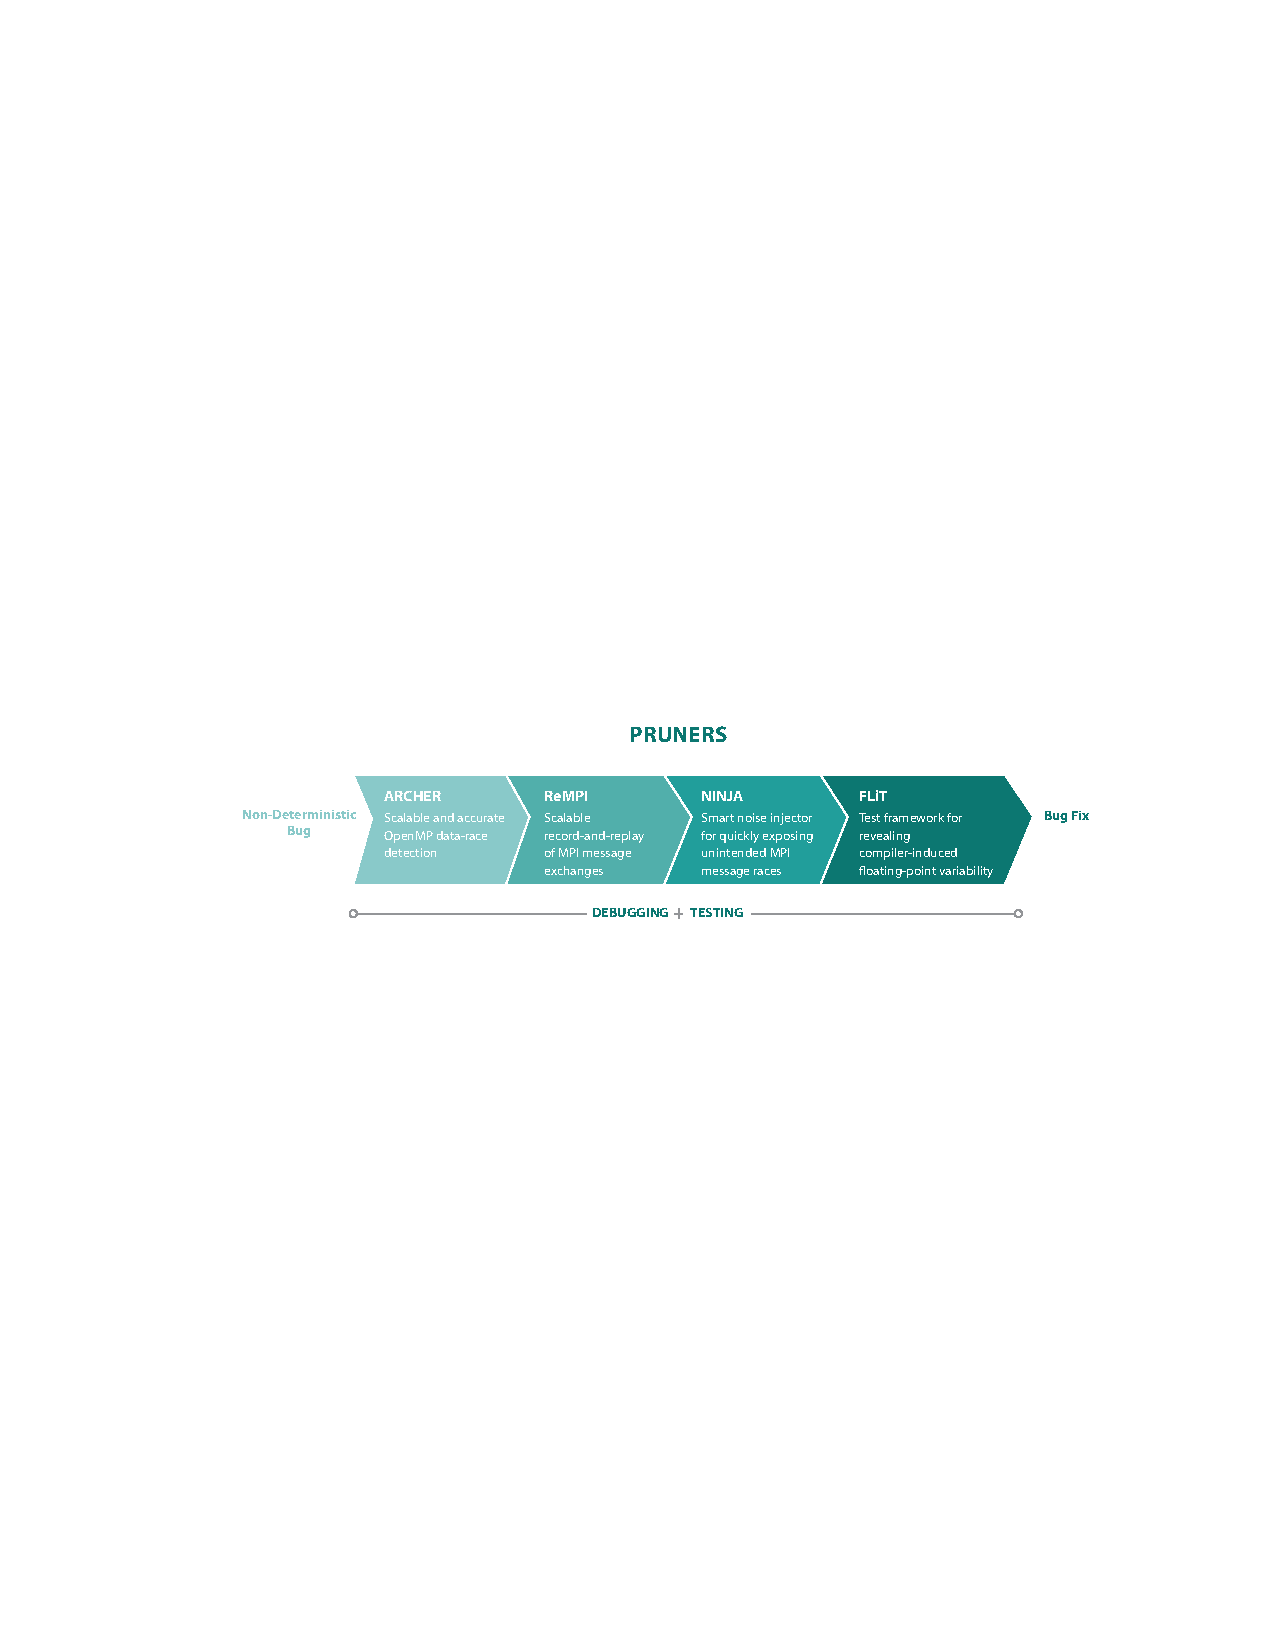
\includegraphics[width=\textwidth]{projects/2.3.6-NNSA/2.3.6.02-LLNL-ATDM/pruners}
\caption{
STAT, Archer, NINJA, and FliT: a continuum of debugging tools for exascale.
}
\end{figure}

Debugging a parallel code can be extremely difficult, and the most
exhaustive approaches for finding errors can require a large amount of
time to run.  For example, understanding all of the potential
interleavings of parallel threaded code requires combinatorial runtime
with respect to the number of threads.  It is not feasible to run this
type of analysis at all times.

Our strategy is to provide a continuum of debugging tools -- from the
lightweight tools like STAT, which require only seconds to run and gives
a high level overview of a code, to Archer, which requires lightweight
code instrumentation, to replay-based fuzzing tools like ReMPI and FLiT,
which run the code in a number of configurations to detect errors.  With
a suite of tools, we can enable developers to find the most common bugs
quickly, while still being able to detect deep, hard-to-find issues given
sufficient runtime and resources.


\paragraph{Recent Progress} \leavevmode \\

\begin{itemize}

\item Completed the port of STAT, Archer, FLiT, ReMPI/NINJA for Sierra,
    deployed them on these systems, and assisted users with these tools for
    debugging and testing.

\item Isolated many elusive bugs for applications running on these systems,
    which includes large-scale code hangs due to NVIDIA GPU for a major ASC code.

\item Archer and ReMPI have been integrated and/or tested with major ASC codes
    and have been running with their verification runs.

\item Started to co-design and harden floating-point correctness checking tools
    (i.e., FLiT and FPChecker) with a large ASC code.

\end{itemize}

\paragraph{Next Steps}  \leavevmode \\

In FY20–FY23, the gap analysis will be completed, and the team will
closely work with the hardware vendors to fill these gaps for El Capitan
and other systems.
